\documentclass[../thesis.tex]{subfiles}

\begin{document}

\chapter{Компоненты системы} \label{chapter:appendix}

Данный раздел подробно описывает компоненты разработанной системы обнаружения.

\section{Proxy}

Основные функции модуля \textit{Proxy} включают:
\begin{enumerate}
\item Перехват OpenFlow сообщений.
\item Установку дополнительных правил маршрутизации.
\item Опрос статистики с коммутаторов.
\end{enumerate}

Proxy реализован с использованием библиотеки \textit{libfluid} \cite{vidal2014libfluid}.
Эта библиотека предоставляет базовые функции для работы с протоколом OpenFlow.
В базовые функции входит обработка сообщений протокола и установка соединений с коммутаторами.
В эту библиотеку также была добавлена логика установки соединений с контроллером.

Вся информация о сети и правилах маршрутизации определяется системой из OpenFlow сообщений, перехватываемых модулем \textit{Proxy}. 
Сбор информации о сети реализован на основе анализа сообщений протокола OpenFlow и, следовательно, не зависит от конкретной реализации контроллера и его приложений.

\section{Handler}

Модуль \textit{Handler} отвечает за обработку OpenFlow сообщений, перехваченных модулем \textit{Proxy}.
Под обработкой понимается следующий набор действий:
\begin{enumerate}
\item Преобразование полей \textit{match}.
\item Модификация устанавливаемых правил
\item Очередизация сообщений от контроллера
\end{enumerate}

\subsubsection{Преобразование полей \textit{match}}

Модуль \textit{Handler} преобразует информацию, полученную из OpenFlow сообщений, в объекты модели \textit{Header Space}.
Поля \textit{match} правил маршрутизации преобразуются в \textit{wildcard} маски, а поля \textit{action} в трансферные функции.

Преобразования также производятся в обратную сторону для создания дополнительных правил маршрутизации.

\subsubsection{Модификация устанавливаемых правил}

Модуль \textit{Handler} сдвигает все правила, устанавливаемые контроллером в сеть, на одну таблицу вперед для того, чтобы использовать нулевые таблицы коммутаторов для установки дополнительных правил маршрутизации.

В сообщениях, идущих от коммутаторов к контроллеру, восстанавливаются оригинальные номера таблиц маршрутизации для того, чтобы не нарушать работу приложений контроллера.

\subsubsection{Очередизация сообщений от контроллера}

OpenFlow сообщения, которые описывают установку правил маршрутизации, изменяют набор ребер в графе зависимостей правил.
При изменении графа зависимостей создаются новые ветви деревьев путевой развертки, и, следовательно, новые дополнительные правила маршрутизации.
Таким образом, при обработке правила $R$ создается список дополнительных правил $\overline{R}_1,\dots,\overline{R}_n$.
Эти дополнительные правила затем будут использоваться системой обнаружения для предсказания значений счетчиков правила маршрутизации $R$.

Если правило $R$ будет установлено в сеть раньше дополнительных правил, то оно успеет обработать некоторое количество пакетов до того, как установятся дополнительные правила.
Следовательно, правила $\overline{R}_1,\dots,\overline{R}_n$ обработают меньшее количество пакетов, чем правило $R$, и во время предсказания значений счетчика правила $R$, произойдет расхождение реального значения счетчика и предсказанного.
Для предотвращения подобной ситуации, дополнительные правила маршрутизации $\overline{R}_1,\dots,\overline{R}_n$ устанавливаются одновременно с правилом $R$.

Для решения проблемы расхождения значений счетчиков модулем\linebreak \textit{Handler} поддерживается очередь сообщений от контроллера.
В этой очереди накапливаются правила, устанавливаемые контроллером.
Сообщения из очереди отправляются в сеть только тогда, когда будут расчитаны соответствующие им дополнительные правила маршрутизации.
Таким образом, дополнительные правила будут установлены на коммутаторы одновременно с оригинальными.

Необходимо отметить, что из-за асинхронности установки правил маршрутизации на разные коммутаторы, эти правила могут установиться не одновременно.
В данном случае расхождение значений счетчиков будет меньше, так как оно зависит от скорости установки правил на коммутаторы, а не от времени построения путевой развертки.

Для учета таких расхождений используется интервал легитимных отклонений, полученный экспериментальным путем.

\section{Network}

Модуль \textit{Network} хранит текущее состояние сети и предоставляет другим модулям \textit{API} к этому состоянию.
Состояние сети описывается при помощи:
\begin{enumerate}
\item Списка коммутаторов.
\item Списка портов.
\item Списка таблиц маршрутизации.
\item Списка правил маршрутизации.
\item Топологии сети.
\end{enumerate}

\section{Dependency Graph}

Основные функции модуля \textit{Dependency Graph} включают:
\begin{enumerate}
\item Построение графа зависимостей правил.
\item Предоставление интерфейса к графу для других приложений.
\end{enumerate}

\subsubsection{Построение графа}

Модуль \textit{Dependency Graph} строит граф зависимостей правил на основе OpenFlow сообщений, перехваченных модулем Proxy.
Граф зависимостей правил изменяется при получении следующих OpenFlow сообщений:
\begin{enumerate}
\item FeaturesReply
\item FlowMod
\item GroupMod
\end{enumerate}

Сообщение \textbf{\textit{FeaturesReply}} отправляется коммутатором на контроллер и содержит информацию о количестве портов и таблиц коммутатора.
Эта информация необходима для создания стоковых и истоковых вершин графа, соответствующих портам коммутатора, а также вершин, соответствующих правилам по-умолчанию в таблицах маршрутизации.

Стоковые вершины описывают входы в сеть, истоковые вершины --- выходы.
Правила по-умолчанию, это правила с наименьшим приоритетом, которые могут обрабатывать пакеты с любыми заголовками, не обработанные другими правилами маршрутизации.
Согласно протоколу OpenFlow \cite{openflow15} такие правила находятся в каждой таблице маршрутизации.
\\

Сообщение \textbf{\textit{FlowMod}} предназначено для установки и удаления правил маршрутизации.
При установке правила, в сообщении указано единственное правило, которое необходимо установить в таблицу маршрутизации коммутатора.
При удалении правила, в сообщении указывается набор параметров, включающий поле \textit{match}.
Коммутатор удаляет все правила маршрутизации, которые описываются этими параметрами, причем удаляются правила, поля \textit{match} которых являются подмножеством поля, указанного в сообщении.

Таким образом, каждое сообщение \textit{FlowMod} приводит либо к созданию единственной вершины графа, либо к удалению набора вершин.
\\

Сообщение \textbf{\textit{GroupMod}} предназначено для установки и удаления групповых правил.
Групповые правила протокола OpenFlow отвечают за групповую маршрутизацию и балансировку нагрузки.
Сообщение \textit{GroupMod} приводит к установке или удалению вершин графа зависимостей правил, соответствующих групповому правилу и набору его \textit{buckets}-записей.

Также на изменение графа влияет обнаружение физических линий, проложенных между коммутаторами.
Обнаружение таких линий происходит при помощи сообщений протокола LLDP, отправляемых коммутаторами на контроллер при помощи \textit{Packet-In} сообщений.

\subsubsection{Интерфейс к графу}

Модуль \textit{Dependency Graph} также предоставляет другим модулям интерфейс к графу зависимостей правил.
Под интерфейсом понимется доступ к вершинам и ребрам графа и возможности прохода по путям графа, с определением заголовков пакетов, которые могут пройти по этому пути.

Интерфейс к графу используется при получении сообщения \textit{Packet-Out} от контроллера.
Эти OpenFlow сообщения указывают коммутатору, что ему нужно сгенерировать пакет на некотором порту или в некоторой потоковой таблице.
Так как сгенерированные пакеты повлияют на значения счетчиков правил маршрутизации, они учитываются при анализе сетевой статистики (рис. \ref{fig:packetout}).

\begin{figure}
\centering
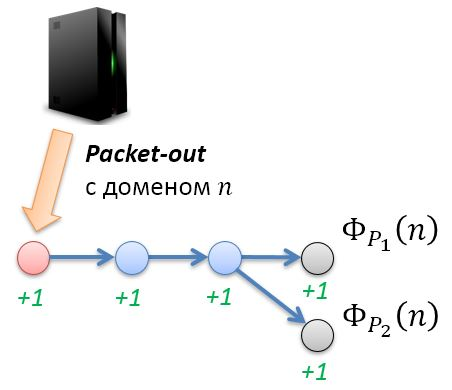
\includegraphics[width=0.4\textwidth]{figures/packetout.jpg}
\caption{Учет сообщений \textit{Packet-Out}} \label{fig:packetout}
\end{figure}

Учет сгенерированных пакетов происходит следующим образом:
\begin{enumerate}
\item Используя заголовок пакета, находится путь, состоящий из правил маршрутизации, который пройдет этот пакет.
\item Значения потоков всех вершин в найденом пути увеличиваются на 1.
\end{enumerate}

Также, при изменении графа зависимостей правил, модуль \textit{Dependency Graph} накапливает список изменений.
Список изменений включает набор добавленных и удаленных ребер графа.
Этот список необходим для того, чтобы изменять путевую развертку только по накопленному набору изменений графа.
Накопление изменений графа позволяет избежать ситуаций, когда удаление и добавление одних и тех же ребер графа приводят к удалению и добавлению одинаковых поддеревьев в путевой развертке.

\section{Flow Predictor}

Основные функции модуля \textit{Flow Predictor} включают:
\begin{itemize}
\item Построение путевой развертки.
\item Предсказание значений счетчиков правил маршрутизации.
\item Установку дополнительных правил маршрутизации.
\item Создание запросов статистики с коммутаторов.
\end{itemize}

Путевая развертка строится на основе списка изменений графа зависимостей правил, полученного из модуля \textit{Dependency Graph}.
После каждого обновления путевой развертки, создается список изменений для дополнительных правил маршрутизации, установленных в сети.
Список изменений представляет собой список с удаляемыми и устанавливаемыми правилами маршрутизации.

\subsubsection{Удаление правил}

При удалении старых правил учитываются ситуации, когда эти правила могли успеть обработать некоторое количество пакетов.
То есть значения счетчиков этих правил маршрутизации не равны нулю.
В данном случае значения счетчиков сохраняются, так как после удаления правил эти значения станут недоступны.

Между отправкой запроса статистики и получением ответа может пройти время, за которое путевая развертка может измениться.
До того момента, как придут ответы статистики по удаляемым правилам, путевая развертка хранит удаленные ветви и, таким образом, представляет собой \textit{персистентную структуру данных} \cite{sarnak1986persistent}.
Персистентная структура данных --- это структура, которая хранит предыдущие состояния и предоставляет к ним доступ.
В данном случае, предыдущими состояниями являются ветви деревьев путевой развертки, соответствующие удаленным доменным путям.

Старые ветви деревьев путевой развертки помечаются флагом \textit{deleted}, но при этом остаются в дереве.
Они не учитываются при построении новых поддеревьев и при вычислении полей \textit{match} новых правил маршрутизации.
Эти ветви используются только для обработки ответов статистики.
Старые ветви удаляются из путевой развертки только после того, как придет последний ответ статистики по удаляемым правилам.

\subsubsection{Обновление путевой развертки}

Также необходимо отметить, что если путевая развертка будет перестраиваться после каждого изменения графа зависимостей правил, может возникнуть ситуация, когда в сети будут устанавливаться и удаляться одни и те же правила маршрутизации.

Такая ситуация может возникнуть, когда контроллер устанавливает путь между двумя хостами в сети.
При установке путей контроллер одновременно устанавливает набор правил, отправляющих пакеты с коммутатора $i$ на коммутатор $i+1$ при $i\in [1,N-1]$.
Эти правила устанавливаются асинхронно, поэтому может возникнуть ситуация, когда они установятся в порядке от первого коммутатора к последнему.

В этой ситуации, в ответ на каждое изменение графа зависимостей правил будет строиться новый доменный путь от клиента к коммутатору $i+1$ и удаляться старый путь к коммутатору $i$.
При этом домены путей к коммутатору $i$ и к коммутатору $i+1$ будут одинаковыми.
А значит и правила, соответствующие этим доменам будут одинаковые.
Таким образом, одни и те же дополнительные правила маршрутизации будут устанавливаться и удаляться $N$ раз.

Так как заранее не известно, какие правила будут устанавливаться в сеть, разработанная система в течение некоторого времени накапливает изменения графа зависимостей правил и только потом перестраивает путевую развертку.
Для этого вводится интервал времени, во время которого накапливаются добавленные и удаленные ребра графа.
По истечении этого интервала вызывается функция, которая использует накопленные изменения для построения путевой развертки и устанавливает в сеть дополнительные правила маршрутизации.
Размер интервала может настраиваться в зависимости от размера сети.

\section{Detector}

Модуль \textit{Detector} производит обнаружение скомпрометированных коммутаторов при помощи информации, предоставляемой модулями \textit{Dependency Graph} и \textit{Flow Predictor}.

Модуль \textit{Detector} использует предсказания значений счетчиков правил маршрутизации, полученные из модуля \textit{Flow Predictor}, и сравнивает эти значения с реальными значениями, запрошенными у коммутаторов.

Если эти значения отличаются, то модуль \textit{Detector} начинает процедуру изменения уровней доверия к коммутаторам.
Процедура заключается в следующем.
\begin{enumerate}
\item Модуль \textit{Detector} использует модуль \textit{Dependency Graph} для того, чтобы найти все пути в графе, проходящие через вершину, соответствующую анализируемому в данный момент правилу маршрутизации.
\item Эти пути используются для обхода всех коммутаторов, которые могли повлиять на потоки, проходящие через анализируемое правило.
\item При обходе модуль \textit{Detector} понижает уровень доверия всех пройденных коммутаторов.
\item Если уровень доверия некоторого коммутатора опускается ниже заданного порога, то модуль сообщает о том, что этот коммутатор скомпрометирован.
\end{enumerate}

Модуль \textit{Detector} также учитывает легитимные потери пакетов, происходящие вследствие перегрузок в сети.
По протоколу OpenFlow, количество всех потерянных пакетов записано в счетчиках на портах коммутаторов.
Модуль \textit{Detector} использует эти счетчики для того, чтобы проверить, что сумма нехватки пакетов по путям, проходящим через некоторый порт, равна количеству пакетов, потерянных на этом порту.
В данном случае, различие счетчиков будет считаться легитимным.

\end{document}